\documentclass[activite]{thedocument}
\usepackage{tabularray}
\startdatakeys
\source{}
\cycle{}
\competencesDuSocle{}
\connaissancesRequises{}
\competencesTravaillees{}
\enddatakeys
\begin{document}
    On considère la fonction $f:x\mapsto1,5x+2$.
    \begin{enumerate}
        \item En utilisant la calculatrice, compléter le tableau ci-dessous.\par\medskip
        \begin{tblr}{colspec=*6{Q[c,m]},column{1}={font=\bfseries},
            vlines,hlines,columns={wd=25pt}}
            $x$&$-4$&$-1,5$&0&2&3\\
            $f(x)$&&&&&\\
        \end{tblr}
        \item En utilisant le tableau ci-dessus, noter d'une croix les points suivants :\par
        $$(-4;f(-4))\hskip10pt(-1,5;f(-1,5))\hskip10pt(0;f(0))\hskip10pt(2;f(2))\hskip10pt(3;f(3))$$
        \vskip10pt
        {\centering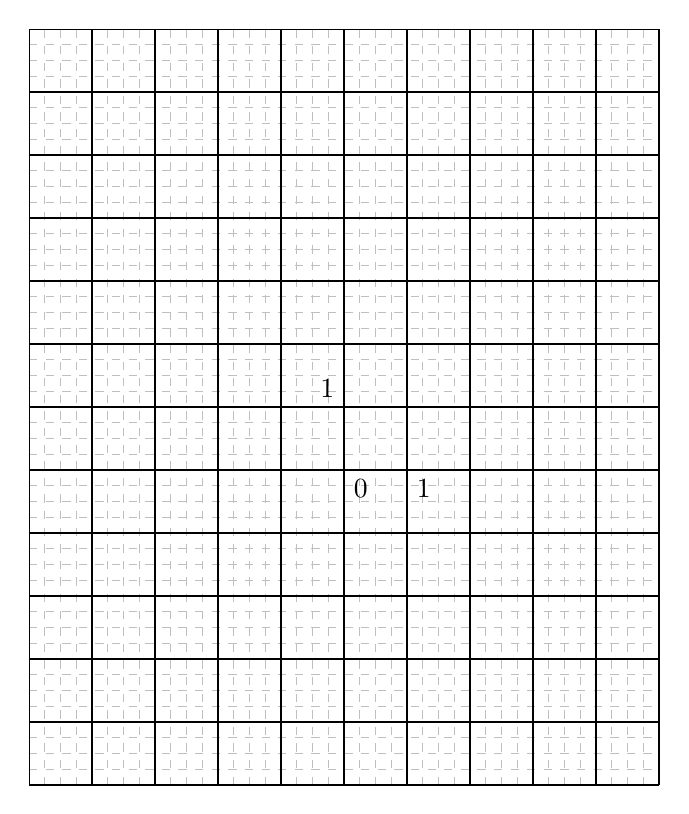
\begin{tikzpicture}[scale=0.8]
            \draw[gray!50!white,step=0.25,dashed](-5,-5)grid(5,7);
            \draw[step=1](-5,-5)grid(5,7);
            \draw[line width=1 pt](-5,0)--(5,0);
            \draw[line width=1 pt](0,-2)--(0,7);
            \draw node[below right]at(0,0){0};
            \draw node[below right]at(1,0){1};
            \draw node[above left]at(0,1){1};
        \end{tikzpicture}\par}
        \item Relier les points du graphique. Comment sont-ils positionnés ?
    \end{enumerate}
\end{document}